% -*- root: ../HistoriaMatematicas.tex -*-
\section{Hoja 1}

Los ejercicios que vienen ahora requieren más búsqueda por internet que otra cosa.

Al final de cada ejercicio añadiré una lista con los link de los que he obtenido la información.

\subsection{Babilonia, Egipto y China}
\begin{problem}[1]
Ejemplos de números escritos por el método babilónico de cuñas

\solution

El sistema de numeración mesopotámica (también llamado numeración babilónica) es un sistema de representación de los números en la escritura cuneiforme de varios pueblos de Mesopotamia, entre ellos los sumerios, los acadios y los babilonios.

Este sistema apareció por primera vez alrededor de 1800-1900  a. C. También se acredita como el primer sistema de numeración posicional, es decir, en el cual el valor de un dígito particular depende tanto de su valor como de su posición en el número que se quiere representar. Esto era un desarrollo extremadamente importante, porque, antes del sistema lugar-valor los técnicos estaban obligados a utilizar símbolos únicos para representar cada potencia de una base (diez, cien, mil, y así sucesivamente), llegando a ser incluso los cálculos más básicos poco manejables.

Aunque su sistema tenía claramente un sistema decimal interno prefirieron utilizar 60 como la segunda unidad más pequeña en vez de 100 como lo hacemos hoy. Más apropiadamente se considera un sistema mixto de las bases 10 y 60. Un valor grande al tener como base sesenta es el número da como resultado un guarismo más pequeño y que además se puede dividir sin resto por dos, tres, cuatro, cinco, y seis, por lo tanto también diez, quince, veinte, y treinta. Solamente dos símbolos usados en una variedad de combinaciones eran utilizados para denotar los 59 números. Un espacio fue dejado para indicar un cero (siglo III a. C.), aunque idearon más adelante una forma de representar un lugar vacío.

La teoría más comúnmente adoptada es que el 60, un número compuesto de muchos factores, fue elegido como base debido a su factorización 2×2×3×5, que lo hace divisible por 1, 2, 3, 4, 5, 6, 10, 12, 15, 20, y 30. De hecho, es el entero más pequeño divisible por todos los enteros del 1 al 6.

Los enteros y las fracciones eran representados de la misma forma: el punto separador de enteros y fracciones no era escritas, sino que quedaban aclaradas por el contexto.


\begin{center}
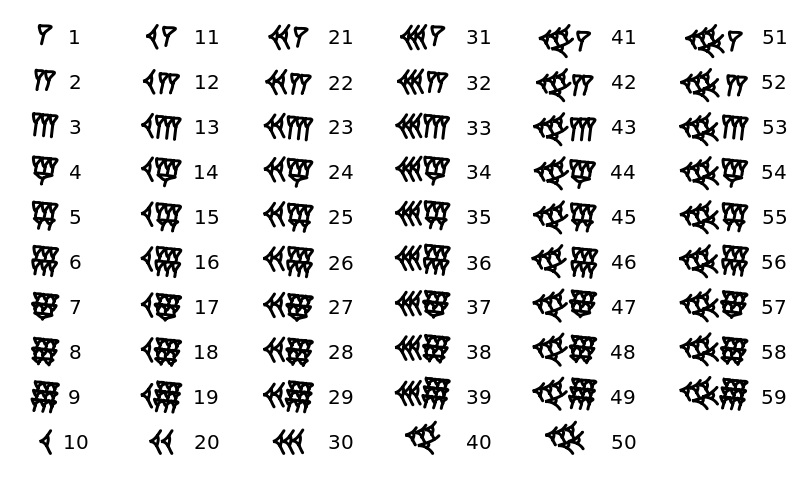
\includegraphics[width=0.8\linewidth]{img/numeros_babilonicos.png}
\end{center}


Por ejemplo, el número 53 en numeración babilónica se representaba utilizando cinco veces el símbolo correspondiente a 10, y 3 veces el símbolo correspondiente a 1, como se puede ver en la imagen superio o solamente el 50 y el 3.

\begin{itemize}
\item \href{https://es.wikipedia.org/wiki/Numeracion_babilonica}{Wikipedia}
\end{itemize}
\end{problem}

\begin{problem}[2]
Ejemplos de números escritos por el método chino tradicional usado hoy día

\solution

La forma clásica de escritura de los números en China se empezó a usar desde el 1500 A.C. aproximadamente. Es un sistema decimal estricto que usa las unidades y los distintas potencias de 10. Utiliza los ideogramas de la figura

\begin{center}
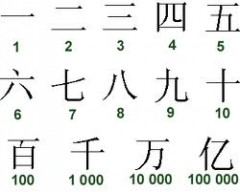
\includegraphics[width=0.4\linewidth]{img/numeracion_china.jpg}
\end{center}

y usa la combinación de los números hasta el diez con la decena, centena, millar y decena de millar para según el principio multiplicativo representar 50, 700 ó 3000. El orden de escritura se hace fundamental,ya que 5 10 7 igual podría representar 57 que 75.

En la

\begin{center}
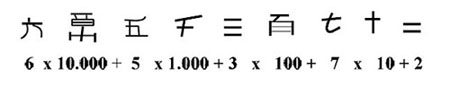
\includegraphics[width=0.6\linewidth]{img/ejemplo_num_chino.jpg}
\end{center}


\begin{itemize}
\item \href{http://www.sectormatematica.cl/historia/chino.htm}{Página random}
\item \href{https://es.wikipedia.org/wiki/Numeracion_china}{Wikipedia}
\end{itemize}
\end{problem}

\begin{problem}[3]
¿Cuál es la mayor terna pitagórica que conocían los babilónicos? Extraer la información de la tablilla Plimton 322

\solution

Plimpton 322 es una tablilla de barro de Babilonia, que destaca por contener un ejemplo de las matemáticas babilónicas. Tiene el número 322 en la colección GA Plimpton en la Universidad de Columbia. Esta tableta, se cree que fue escrita cerca de 1800 a. C., tiene una tabla de cuatro columnas y 15 filas de números en escritura cuneiforme de la época.

Esta tabla muestra lo que ahora se llaman ternas pitagóricas, es decir, números enteros a, b, c que satisfacen $a^2+b^2=c^2$. Las tripletas son demasiadas como para haber sido construidas por fuerza bruta (es decir, hechas a mano probando valores).

Desde una perspectiva moderna, un método para construir tales tripletas es un primer logro significativo, conocido antes sólo entre los griegos . Al mismo tiempo, hay que recordar que el autor de la tableta era un escriba, más que un matemático profesional, se ha sugerido que uno de sus objetivos pueden haber sido producir ejemplos para problemas escolares.

Aunque la tableta se interpretó en el pasado como una tabla trigonométrica, más recientemente se han publicado trabajos que ven esto como un anacronismo, y le dan una función diferente.

El contenido principal de Plimpton 322 es una tabla de números, con cuatro columnas y quince filas, en notación sexagesimal babilónica. La cuarta columna es sólo un número de fila, ordenada del 1 al 15. Las segunda y tercera columnas son completamente visible en la tableta sobreviviente. Sin embargo, el borde de la primera columna se ha roto, y existen dos extrapolaciones consistentes que dan los dígitos faltantes que podrían haber sido; estas interpretaciones difieren sólo en si cada número comienza con un dígito adicional igual a 1 o no. Con las diferentes extrapolaciones mostradas en paréntesis, estos números son:

Si traducimos la tabla literalmente tenemos
\begin{center}
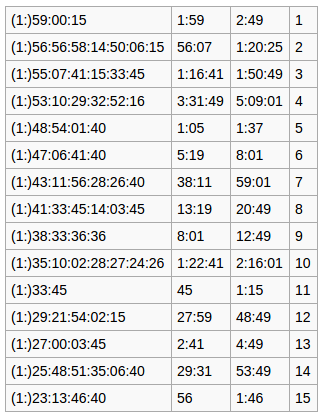
\includegraphics[width=0.5\linewidth]{img/plimton_literal.png}
\end{center}

que se interpreta como:
\begin{center}
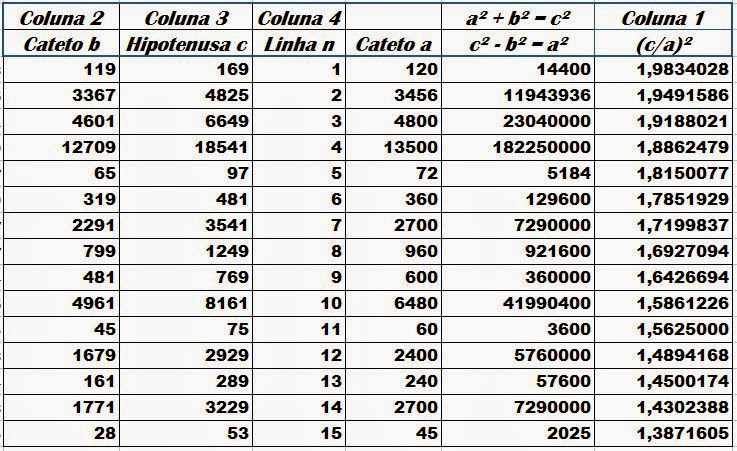
\includegraphics[width=0.8\linewidth]{img/plimton322.jpg}
\end{center}

En respuesta al ejercicio, la terna más grande que conocían es
\[(13500, 12709, 18541)\]

\begin{itemize}
\item \href{https://es.wikipedia.org/wiki/Plimpton_322}{Wikipedia}
\end{itemize}

\end{problem}

\begin{problem}[4]
Raíz cuadrada por el \textbf{método de Heron}.

Sea
\[x_{n+1} = \frac{1}{2} \left(x_n + \frac{R}{x_n} \right)\]
demostrar que existe el límite y que la serie converge a  $\sqrt{R}$. Describir el conjunto de los datos iniciales que llevan a convergencia.
\solution

\doneby{Pedro}

El método de Herón que menciona el ejercicio es un algoritmo que nos permite calcular raíces cuadradas (más bien aproximaciones a las mismas).

Para estudiar la convergencia podemos buscar el punto fijo de la ecuación.
\[x_n = \frac{1}{2} \left(x_n+\frac{R}{x_n}\right) \implies \frac{1}{2}x_n=\frac{1}{2}\frac{R}{x_n} \implies x_n^2=R \implies x_n = \sqrt{R}\]

El método funcionará (convergerá a lo que deseamos) si
\[\norm{f(x)-f(y)} \leq K \norm{x-y} \text{ con } f(x)=\frac{1}{2} \left( x + \frac{R}{x} \right)\]

Podemos ver que
\[\norm{f(x)-f(y)} = \frac{R}{2}\left(\frac{1}{x}-\frac{1}{y}\right)\]

Sea $x$ la solución, es decir $x=\sqrt{R}$ podemos escribir $y=x+ε$ lo que nos lleva a:
\[\norm{f(x)-f(y)} = \frac{R}{2}\left(\frac{1}{x}-\frac{1}{x+ε}\right) = \frac{R}{2} \left( \frac{ε}{x^2+xε} \right)<Kε\]

Para garantizar la desigualdad necesitamos que el denominador sea mayor que 1, es decir, basta con tomar
\[x^2+xε > 1 \implies ε > \frac{1-x^2}{x}=\frac{1-R}{\sqrt{R}}>\frac{1}{\sqrt{R}}-\sqrt{R}\]

Por tanto basta con que tomemos un punto $y>x+\frac{1}{\sqrt{R}}-\sqrt{R} = \frac{1}{\sqrt{R}}$.

Cuando $R$ sea bastante grande, prácticamente nos bastará con tomar cualquier número positivo.


\end{problem}

\subsection{Grecia}
\begin{problem}[5]
Elaborar una tabla con el alfabeto griego, los símbolos, la fonética y el nombre y pronunciación usual de cada letra.

\obs Epsilon y eta; i e ípsilon; o y omega; zeta y theta; nu, xi, phi, psi y los diptongos ai=e, ei=i

\solution

El alfabeto griego es un alfabeto de veinticuatro letras utilizado para escribir la lengua griega. Desarrollado alrededor del siglo IX a. C. a partir del alfabeto consonántico fenicio, los griegos adoptaron el primer alfabeto completo de la historia, entendiéndolo como la escritura que expresa los sonidos individuales del idioma, es decir que prácticamente a cada vocal y cada consonante corresponde un símbolo distinto.

\begin{center}
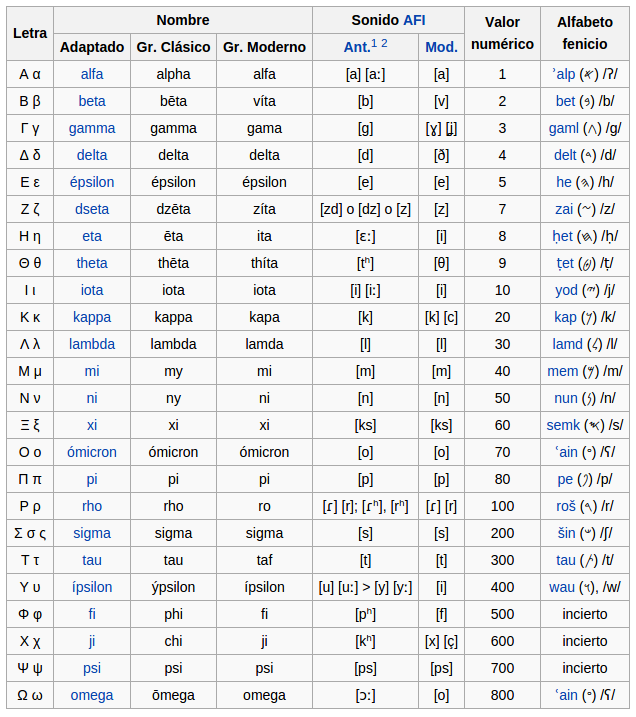
\includegraphics[width=0.5\linewidth]{img/alfabeto_griego.png}
\end{center}


Su uso continúa hasta nuestros días, tanto como alfabeto nativo del griego moderno como a modo de crear denominaciones técnicas para las ciencias, en especial la lógica, la matemática, la física, la astronomía y la informática.


\begin{itemize}
\item \href{https://es.wikipedia.org/wiki/Alfabeto_griego}{Wikipedia}
\end{itemize}


\end{problem}

\subsection{Thales}
\begin{problem}[6]
\ppart Demostrar que en un triángulos con dos lados iguales hay dos ángulos iguales y viceversa

\ppart Demostrar que la suma de ángulos de un triángulo es un ángulo plano

\ppart Demostrar el siguiente teorema de Tales: el ángulo inscrito en una semicircunferencia es recto. Demostrar el inverso

\ppart Demostrar que el ángulo inscrito en una circunferencia vale la mitad del ángulo central correspondiente

\solution

\doneby{Pedro}

\spart

Si tomamos un triángulo isósceles podemos dividirlo en dos triángulos rectángulos dibujando la altura sobre el lado desigual.

Asumiendo que los lados son iguales, vamos a obtener dos triángulos con los tres lados iguales por lo que también tendrán los ángulos iguales.

\spart

Basándonos en el Teorema de Tales tenemos:

\begin{center}
\inputtikz{suma_angulos_triangulo}
\end{center}

donde las rectas del mismo color son paralelas y los del mismo color iguales por el teorema de tales.

Viendo esto y sabiendo que un ángulo llano tiene 180 grados, es sencillo ver que la suma de los ángulos es 180.

\spart


\end{problem}

\subsection{Pitágoras}
\begin{problem}[7]
Escribir la definición de las ternas pitagóricas. Describir todas las ternas pitagórigas mediante dos fórmulas. Listar todas aquellas ternas que tienen todos los números menores que 500

\solution

Una terna pitagórica consiste en una tupla de tres enteros positivos a, b, c que cumplen que a² + b² = c². El nombre deriva del teorema de Pitágoras, el cual plantea que en cualquier triángulo rectángulo, se cumple que x² + y² = z² (siendo x e y las longitudes enteras de sus catetos y z la de la hipotenusa). En sentido contrario también se cumple, o sea, cualquier terna pitagórica se puede asociar con las longitudes de dos catetos y una hipotenusa, formando un triángulo rectángulo.

Las ternas pitagóricas suelen representarse como (a,b,c).



\begin{itemize}
\item \href{https://conlamenteabierta.wordpress.com/2010/02/18/diofanto-y-las-tripletas-pitagoricas/}{CONLAMENTEABIERTA}
\end{itemize}
\end{problem}

\begin{problem}[8]
Método de Diofanto para calcular las ternas pitagóricas. Describir el método y el uso de los números fraccionarios.

Aplicar el método disparando de $N=(0,-1)$ o desde $N'=(1,0)$. Comparar

\solution

Una relación que nos dio Diofanto para calcular ternas pitagóricas es:

\[\left\{ \begin{array}{l} a=p^2-q^2 \\ b=2pq \\ c=p^2+q^2 \end{array} \right.\]

Considerando los datos iniciales del enunciado tenemos:
\[N \to (-1,0,1); \ \ N' \to (-1,0,1)\]

Obtenemos el mismo resultado en ambos casos pues las magnitudes aparecen elevadas al cuadrado.

\begin{itemize}
\item \href{https://en.wikipedia.org/wiki/Diophantus_II.VIII}{Wikipedia en inglés}
\end{itemize}
\end{problem}

\begin{problem}[9]
Leer el capítulo 1 de Stillwell (3rd Edition). Hacer los ejercicios 1.2.{1,3,4}, 1.2.4, 1.3.{1,2,3}.

Especialmente el último

\solution

\end{problem}

\begin{problem}[10]
Sea $(a,b,c)$ una terna pitagórica generada por $(p,q)$ con $a,b,c,p,q$ enteros positivos, demostrar que si $p=q+1$, entonces $c=b+1$.

\solution
\doneby{Pedro}

Recordemos que las ternas pitagóricas podrían generarse a partir de dos enteros $p$ y $q$ considerando:
\[\left\{ \begin{array}{l} a=p^2-q^2 \\ b=2pq \\ c=p^2+q^2 \end{array} \right.\]

Si tomamos $p=q+1$ obtendremos
\[c=p^2+q^2=(q+1)^2-q^2=1+2q+2q^2\]
Por otro lado tendremos:
\[b=2pq=2(q+1)q=2q^2+2q\]
Así es sencillo ver que
\[c=b+1\]
\end{problem}

\begin{problem}[11]
Demuestra que al menos uno de los tres términos de una terna pitagórica es par.

\solution

\doneby{Pedro}

Si ninguno fuese par, tendríamos que todos los cuadrados son impares y al escribir:
\[a^2+b^2=c^2\]
tendríamos que la suma de dos números impares es impar, afirmación que es totalmente falta.
\end{problem}

\begin{problem}[12]
\ppart En toda terna pitagórica generada por $p$ y $q$ siendo ambos positivos y $p>q$, mediante la fórmula simple
\[F(p,q)=(p^2-q^2,2pq,p^2+q^2)\]
al menos uno de los tres números resultantes es divisible por 3.

\ppart En toda terna pitagórica $(a,b,c)$ generada por $p$ y $q$ como antes, al menos uno de los tres números resultantes es divisible por 5
\solution

\doneby{Pedro}

\spart

Supongamos que ninguno de los números es múltiplo de 3, es decir:
\[\left\{ \begin{array}{l} a=p^2-q^2=3m+i \\ b=2pq=3n+j \\ c=p^2+q^2=3h+k \end{array} \right. \text{con } i,j,k = 1 \text{ ó } 2\]

Cuando pasemos a corroborar que se satisface la ecuación de Pitágoras tendremos:
\[9m^2+i^2-6mi+9n^2+j^2+6nj=9h^2+k^2+6hk\]

Podemos ver que $i^2,j^2,k^2=3l+1$ con $l=1 \text{ ó } 0$.

Por tanto, agrupando los múltiplos de 3 a ambos lados nos quedará:
\[3x+2=3y+1\]
igualdad que no puede satisfacerse siendo $x,y$ enteros.

\spart

Repetimos el mismo procedimiento del apartado anterior.

Supongamos que ninguno de los números es múltiplo de 5, es decir:
\[\left\{ \begin{array}{l} a=p^2-q^2=5m+i \\ b=2pq=5n+j \\ c=p^2+q^2=5h+k \end{array} \right. \text{con } i,j,k = 1,2,3 \text{ ó } 4\]

Cuando pasemos a corroborar que se satisface la ecuación de Pitágoras tendremos:
\[25m^2+i^2-10mi+25n^2+j^2+10nj=25h^2+k^2+10hk\]

Podemos ver que $i^2,j^2,k^2=5l+t$ con $t=1 \text{ ó } 4$.

Por tanto, agrupando los múltiplos de 5 a ambos lados nos quedará:
\[5x+u=5y+v\]

Veamos todos los casos posibles.
\begin{center}
\begin{tabular}{|c|c|c|}
\hline
u & v & Validez\\
\hline
\hline
2 & 1 & No \\
 \hline
5 & 1 & No \\
 \hline
3 & 1 & No \\
\hline
2 & 4 & No \\
 \hline
5 & 4 & No \\
 \hline
3 & 4 & No \\
\hline
\end{tabular}
\end{center}

Podemos ver que en ningún caso se puede satisfacer la ecuación.

\end{problem}

\begin{problem}[13]
Hallar una terna pitagórica especial que genere un triángulo rectángulo cuyas alturas sean, todas ellas, números enteros positivos
\solution

\doneby{Pedro}

Puesto que hablamos de triángulos rectángulos, los lados $a$ y $b$ ya son alturas entre ellos.

Por tanto, toda terna pitagórica nos da un triángulo en el que dos de sus alturas son números enteros positivos.

Sabemos calcular el área de un triángulo rectángulo de dos formas distintas que deben dar el mismo valor:
\[A = \frac{bc}{2} = \frac{ah}{2} \implies h = \frac{bc}{a}\]

donde $h$ es justo la altura de la que no podemos garantizar que sea entera.

Tanteando un poco parece lógico tomar valores de $p$ y $q$ que tengan un factor común y si ese factor común es el $2$ parece que será más sencillo puesto que al generar la $b$ nos aparece un 2.

Finalmente, por la cuenta de la vieja podemos ver que
\[p=10, \ q=6\left\{ \begin{array}{l} a=p^2-q^2=64=2^(6) \\ b=2pq=120=2^3(5\cdot 3) \\ c=p^2+q^2=136=2^3\cdot 17 \end{array} \right. \]

Y podemos comprobar fácilmente que este caso satisface que $h=\frac{bc}{a} \in \nat$.
\end{problem}

\begin{problem}[14]
Hacer los ejercicios 1.5.{1,2} del Stillwell
\solution

\end{problem}

\begin{problem}[15]
Teorema de Pitágoras. Enunciado e interpretación geométrica. Dos pruebas por la técnica de recorte de figuras (tangram)
\solution

Este ejercicio esta resuelto en la teoría, concretamente en los apartados \ref{sec:Prueba1} y \ref{sec:Prueba2}
\end{problem}

\begin{problem}[16]
Teorema de Pitágoras. Enunciado y prueba por el Método de Semejanzas. Obtener los dos teoremas de la altura.

\solution

Este ejercicio está resuelto en la teoría, concretamente en \ref{sec:Prueba3}


\end{problem}

\subsection{Construcciones geométricas}
\begin{problem}[17]
\ppart Construcciones con regla y compás: Dividir un segmento en 2,3,...,p partes iguales.
\ppart Hallar un trozo de segmento dado en proporción m/n al total
\ppart Hallar un trozo de un segmento dado en la proporción $\frac{1}{\sqrt{2}}$

\solution

\end{problem}

\begin{problem}[18]
Construcciones con regla y compás. Construir un cuadrado equivalente a un rectángulo dado. Construir un cuadrado de área dada.
\solution

\end{problem}

\begin{problem}[19]
Hacer los cálculos de longitudes y áreas en los polígonos regulares de 3, 4, 6 y 8 lados. Intentarlo con el pentágono.
\solution

\end{problem}

\begin{problem}[20]
Problemas de axiomas y modelos. Examinar si en los postulados de Euclides se puede cambiar recta por punto y viceversa y obtener unos axiomas válidos
\solution

\end{problem}


\begin{problem}[21]
Explicar cuál es el problema histórico del V Postulado
\solution

\end{problem}

\subsection{Aritmética}
\begin{problem}[22]
Calcular la fórmula de los números triangulares y pentagonales
\solution

\end{problem}

\begin{problem}[23]
EUCLIDES: Números primos: algoritmo para la descomposición de un número entero positivo en producto de números primos. Demostración de unicidad. Teorema de Bezout.
\solution

\end{problem}

\begin{problem}[24]
Algoritmo de Euclides para el m.c.d. Aplicar el algoritmo para una pareja de números dados.
\solution

\end{problem}

\begin{problem}[25]
Demostración de infinitud de los números primos
\solution

\end{problem}

\begin{problem}[26]
Demostración de que el número $e$ no es racional.
\solution

\end{problem}